\chapter{Contexte général du projet}
    
\rhead{Contexte général du projet}
\lfoot{\leftmark}

\section{Introduction}
Ce chapitre a pour objectif de définir le cadre dans lequel s'inscrit le projet de fin d'études. Nous commençons par présenter le contexte général et la problématique à laquelle répond le projet, avant de détailler la solution proposée, les objectifs visés, les livrables attendus ainsi que les spécifications des besoins. Enfin, nous abordons la méthodologie adoptée et la planification du projet.

%--------------------------1-----------------------------
\section{Contexte du projet}
Le projet Apache Spark \cite{logo:apache_spark}, géré via la plateforme JIRA \cite{logo:jira_apache} de la fondation Apache, figure parmi les initiatives open source les plus dynamiques dans l'écosystème du traitement distribué. Au fil des années, ce projet a généré un volume considérable de tickets, avoisinant les 50 000 entrées, de natures très diverses : signalements d'anomalies, demandes d'amélioration, ajouts de fonctionnalités, tâches techniques, sous-tâches, interrogations ou encore éléments de documentation. Chacun de ces tickets s'accompagne d'un ensemble dense de métadonnées : un intitulé synthétique, un descriptif parfois très long, des fils de commentaires, un journal de modifications traçant chaque changement de champ, des liaisons vers d'autres tickets, sans oublier les informations relatives à la priorité, au statut courant, à la personne ayant signalé le problème et à celle chargée de le traiter.

Dans un tel environnement, l'activité de triage, c'est-à-dire la catégorisation et l'orientation de chaque nouveau ticket, représente un enjeu opérationnel majeur. Il s'agit concrètement de déterminer la nature exacte du ticket, d'estimer comment il sera vraisemblablement résolu et de formuler une piste d'action pour les développeurs. Aujourd'hui, cette tâche incombe principalement à des contributeurs expérimentés qui l'effectuent manuellement, ce qui consomme un temps non négligeable et reste exposé aux aléas de l'interprétation humaine, surtout lorsque le flux de tickets s'intensifie.

% Notre travail prolonge l'expérience acquise lors du hackathon Data \& IA organisé par SQLI, au cours duquel une première approche de triage hybride a été explorée à l'aide de Snowflake Cortex. L'ambition est ici de passer d'un prototype à une plateforme industrialisée et enrichie. Les données exploitées proviennent d'un export public du JIRA Apache Spark, mis à disposition sur Kaggle en mars 2025. Cet export totalise environ 49 832 tickets pour le projet SPARK, auxquels sont associés plus de cinq millions de commentaires, 9,6 millions d'entrées dans le journal de modifications et 390 000 relations entre tickets.

%------------------------2--------------------------
\section{Étude de l’existant}
Plusieurs stratégies ont été documentées dans la littérature et dans la pratique pour aborder la question du triage automatique des incidents logiciels. Nous en distinguons quatre grandes familles.
\begin{itemize}
    \item La première, et la plus couramment observée dans les projets open source de grande envergure, est le triage entièrement manuel. Des contributeurs chevronnés parcourent les tickets un par un, les catégorisent selon leur expérience et les affectent aux personnes compétentes. Si cette méthode bénéficie d'une connaissance fine du contexte technique, elle présente des faiblesses structurelles : le temps consacré à chaque ticket est élevé, la disponibilité des experts conditionne le rythme de traitement, les critères de classification varient d'un triageur à l'autre, et les épisodes de forte affluence engendrent des retards cumulatifs.
    \item La deuxième famille regroupe les techniques d'apprentissage automatique supervisé dites classiques. Des algorithmes tels que les séparateurs à vaste marge, les ensembles d'arbres de décision ou les classifieurs probabilistes sont alimentés par des vecteurs de caractéristiques construits manuellement à partir du texte des tickets, par exemple via des représentations en sacs de mots ou en pondérations TF-IDF \cite{logo:tfidf}. Ces méthodes ont produit des résultats intéressants sur des corpus de taille modeste, mais elles peinent à saisir les nuances sémantiques des descriptions techniques et exigent un investissement conséquent dans la phase de construction des caractéristiques.
    \item La troisième famille s'appuie sur les grands modèles de langage. Grâce à leur capacité à appréhender le sens contextuel de textes spécialisés, ces modèles offrent des performances de classification et de génération nettement supérieures. Toutefois, leur mise en œuvre directe pour le triage soulève des questions de coût computationnel, de temps de réponse et de contrôle de la qualité des sorties, notamment lorsqu'il faut garantir des prédictions cohérentes sur des milliers de tickets.
    \item La quatrième famille, qualifiée d'hybride, associe une recherche par similarité vectorielle à un arbitrage par modèle de langage, selon le principe du Retrieval-Augmented Generation (RAG) \cite{logo:rag}. Son intérêt réside dans la complémentarité entre la rapidité de la recherche par plus proches voisins et la finesse de raisonnement du modèle de langage, le tout encadré par un mécanisme de seuil de confiance qui réserve les appels coûteux au LLM aux seules situations véritablement ambiguës.
\end{itemize}

Au terme de cette analyse, il ressort qu'aucune solution opérationnelle ne fédère dans une même architecture l'ensemble de la chaîne nécessaire : ingestion, transformation, enrichissement par des indicateurs issus de l'historique de modifications et des relations inter-tickets, classification hybride et production d'analyses correctives, le tout hébergé sur une plateforme cloud unifiée.

%------------------------3-------------------------
\section{Problématique}
Le processus de triage des incidents du projet Apache Spark repose, dans sa forme actuelle, sur une intervention humaine systématique. Les responsables qualité doivent lire chaque ticket dans son intégralité, en identifier la nature, projeter son issue probable et orienter les équipes de développement. Avec un historique de près de 50 000 tickets et un flux continu de nouvelles entrées, cette organisation atteint ses limites. Nous identifions trois difficultés majeures.

\begin{itemize}
    \item La première touche au coût temporel du diagnostic. L'examen approfondi d'un ticket complexe, englobant sa description, ses commentaires et l'intégralité de son journal de modifications, peut s'avérer particulièrement chronophage, a fortiori lorsque le ticket a fait l'objet de multiples réassignations ou d'escalades de priorité.
    \item La deuxième difficulté concerne l'hétérogénéité des classifications. Sans règles formalisées ni assistance automatisée, deux triageurs confrontés au même ticket peuvent aboutir à des catégorisations divergentes, ce qui nuit à la cohérence du suivi et fausse l'analyse des tendances sur le long terme.
    \item La troisième difficulté porte sur la sous-exploitation des métadonnées disponibles. Le journal de modifications recèle des informations précieuses, telles que la fréquence des transitions de statut, les hausses de priorité ou la diversité des intervenants, qui constituent autant d'indices sur la complexité et la criticité d'un ticket. Or, ces signaux ne sont aujourd'hui intégrés dans aucune démarche de triage existante.
\end{itemize}

La question centrale à laquelle ce projet entend répondre est la suivante : comment élaborer et déployer une plateforme intégrée permettant d'automatiser le triage des incidents Apache Spark, en valorisant la totalité des données JIRA disponibles, dans le but de prédire la catégorie de l'incident et son issue probable, tout en proposant une analyse corrective directement exploitable par les équipes ?

%------------------------4-------------------------
\section{Solution proposée}
Pour répondre à cette problématique, nous proposons la conception et le déploiement d'une plateforme de triage automatique reposant sur une architecture en médaillon à trois niveaux (Bronze, Argent, Or) \cite{logo:medallion}, hébergée intégralement sur Snowflake \cite{logo:snowflake} et orchestrée par dbt \cite{logo:dbt}.

La couche Bronze prend en charge l'ingestion fidèle des données brutes issues des fichiers CSV sources, sans aucune transformation métier, afin de préserver l'intégralité de l'information d'origine.

La couche Argent porte l'essentiel de la logique de transformation. Elle assure le filtrage, le nettoyage textuel, la consolidation des étiquettes en catégories exploitables, le partitionnement temporel des données, ainsi que l'extraction de caractéristiques originales à partir du journal de modifications et des relations entre tickets. Ces caractéristiques constituent l'apport technique distinctif de ce projet.

La couche Or produit les tables de consommation finales, alimentant d'une part le pipeline de classification et d'autre part le tableau de bord analytique.

Le moteur de classification s'appuie sur une approche hybride combinant une recherche par similarité vectorielle avec un arbitrage par modèle de langage lorsque le niveau de confiance est insuffisant. Ce pipeline produit, pour chaque ticket, une prédiction du type d'incident, une prédiction de la résolution probable et un résumé correctif court.

La plateforme expose deux canaux de restitution : une application de triage en temps réel développée avec Streamlit \cite{logo:streamlit}, et un tableau de bord analytique multi-pages permettant l'exploration des données opérationnelles. Les détails de conception et d'implémentation de chacune de ces couches seront approfondis dans les chapitres suivants.

%------------------------5-------------------------
\section{Objectifs du projet}
Ce projet poursuit un objectif principal et plusieurs objectifs spécifiques.

L'objectif principal est de concevoir et de mettre en service une plateforme de bout en bout automatisant le triage des incidents Apache Spark, couvrant l'intégralité de la chaîne, depuis l'ingestion des données brutes jusqu'à la restitution des prédictions et des analyses.
Pour les objectifs spécifiques
\begin{itemize}
    \item Le premier consiste à bâtir une architecture en médaillon fiable sur Snowflake, pilotée par dbt, dans laquelle chaque transformation est tracée et validée par des tests automatisés.
    \item Le deuxième vise à extraire et intégrer des caractéristiques inédites issues du journal de modifications et des liaisons entre tickets. 
    \item Le troisième objectif porte sur le calibrage du pipeline de classification hybride pour dépasser un taux de classification correcte de 70 \% sur le type d'incident et de 75 \% sur la résolution. 
    \item Le quatrième objectif consiste à développer une interface de triage en temps réel et un tableau de bord d'analyse accessibles aux responsables qualité.
    \item Le cinquième objectif est d'assurer la reproductibilité intégrale de la solution au moyen d'une documentation exhaustive et d'un déploiement par conteneurs.
\end{itemize}
%------------------------6-------------------------
\section{Livrables attendus}
Le projet doit aboutir à la production de sept livrables distincts.
\begin{itemize}
    \item Le premier est la base de données Snowflake organisée selon l'architecture en médaillon, comprenant six schémas dédiés aux différentes couches de transformation et de consommation.
    \item Le deuxième est le projet dbt dans son intégralité, englobant les modèles de transformation pour chaque couche, les tables de correspondance pour le regroupement des étiquettes, les macros de nettoyage textuel et la batterie de tests automatisés.
    \item Le troisième est le pipeline V6 Hybrid RCA, matérialisé par quatre scripts SQL séquentiels couvrant l'enrichissement, le calcul des représentations vectorielles, la prédiction et l'évaluation.
    \item Le quatrième est l'application de triage en temps réel, développée avec Streamlit, offrant pour chaque ticket soumis une prédiction du type, de la résolution et un résumé correctif.
    \item Le cinquième est le tableau de bord analytique multi-pages, permettant l'exploration des données opérationnelles et des relations entre tickets.
    \item Le sixième est la documentation technique, comprenant le dictionnaire des données, le journal des décisions architecturales et le schéma global de la plateforme.
    \item Le septième est l'environnement de déploiement conteneurisé, permettant le lancement de l'ensemble des applications par une commande unique.
\end{itemize}

%------------------------7-------------------------
\section{Spécification des besoins}
\subsection{Besoins fonctionnels}
 la plateforme doit être capable d'ingérer les données JIRA Apache Spark depuis des fichiers CSV et de les charger dans Snowflake en préservant l'intégralité de l'information. Elle doit appliquer aux données brutes un traitement comprenant un nettoyage textuel, une consolidation des étiquettes et un partitionnement temporel. Elle doit calculer des indicateurs à partir du journal de modifications, notamment le nombre de transitions de statut, les variations de priorité, les changements d'assignataire, la détection des escalades et le dénombrement des intervenants uniques. Elle doit également dériver des indicateurs à partir des relations entre tickets, incluant les doublons, les blocages et les liens de type informationnel. La plateforme doit attribuer à chaque ticket une catégorie parmi neuf classes de type et une parmi sept classes de résolution. Elle doit produire un résumé correctif concis pour chaque prédiction. Elle doit mettre à disposition une interface de triage en temps réel pour un ticket individuel, ainsi qu'un tableau de bord interactif couvrant les dimensions opérationnelles et relationnelles des tickets.

\subsection{Besoins non fonctionnels}
la plateforme doit garantir un taux de classification correcte dépassant 70 \% pour le type d'incident et 75 \% pour la résolution. La fiabilité des transformations doit être assurée par des tests dbt automatisés portant sur l'unicité des clés, l'absence de valeurs manquantes sur les champs critiques, le respect des valeurs autorisées et la cohérence des relations entre tables. La confidentialité doit être respectée en maintenant une version locale de développement séparée de l'environnement de production de l'entreprise. L'ensemble de la solution doit pouvoir être reproduit et déployé via un système de conteneurisation. Le pipeline principal de classification doit s'appuyer exclusivement sur les modèles accessibles via Snowflake Cortex, sans recourir à des services tiers. Enfin, le code source et la documentation doivent faire l'objet d'un suivi de versions sur un dépôt distant.

%------------------------8-------------------------
\section{Méthodologie et gestion du projet}
\subsection{Choix de la méthode de gestion du projet}

La conduite du projet s'appuie sur une démarche itérative et incrémentale, inspirée du cadre Scrum tel que pratiqué au sein de SQLI. Ce choix permet de livrer progressivement les différentes briques de la plateforme, en ménageant à chaque itération des moments de revue et d'ajustement avec l'encadrant en entreprise.

Le processus Scrum\cite{logo:SCRUM}, représenté à la Figure~\ref{fig:scrum}, suit les étapes suivantes :

\begin{description}
    \item[Identification des fonctionnalités] à développer pour construire le backlog produit (ingestion des fichiers CSV dans Snowflake, nettoyage et transformation des données via dbt, extraction des features du changelog et des liens entre tickets, mise en place du pipeline de classification hybride, développement de l'application d'inférence Streamlit, création du tableau de bord analytique, conteneurisation via Docker).
    \item[Priorisation des tâches] à travers des sprints successifs, en tenant compte de la complexité technique et des dépendances entre composants.
    \item[Développement itératif] où chaque sprint aboutit à un incrément fonctionnel du produit, tel qu'une couche Bronze opérationnelle avec tests de validation, un pipeline dbt complet produisant la table mart_ml, un premier prototype du pipeline de classification ou encore un tableau de bord avec les premières visualisations.
\end{description}

Cette approche m'a permis de progresser de façon organisée et adaptable, en passant par des étapes bien définies telles que la planification des tâches, le développement itératif et les tests, ainsi que l'intégration continue des composants. 

\begin{figure}[H]
    \centering
    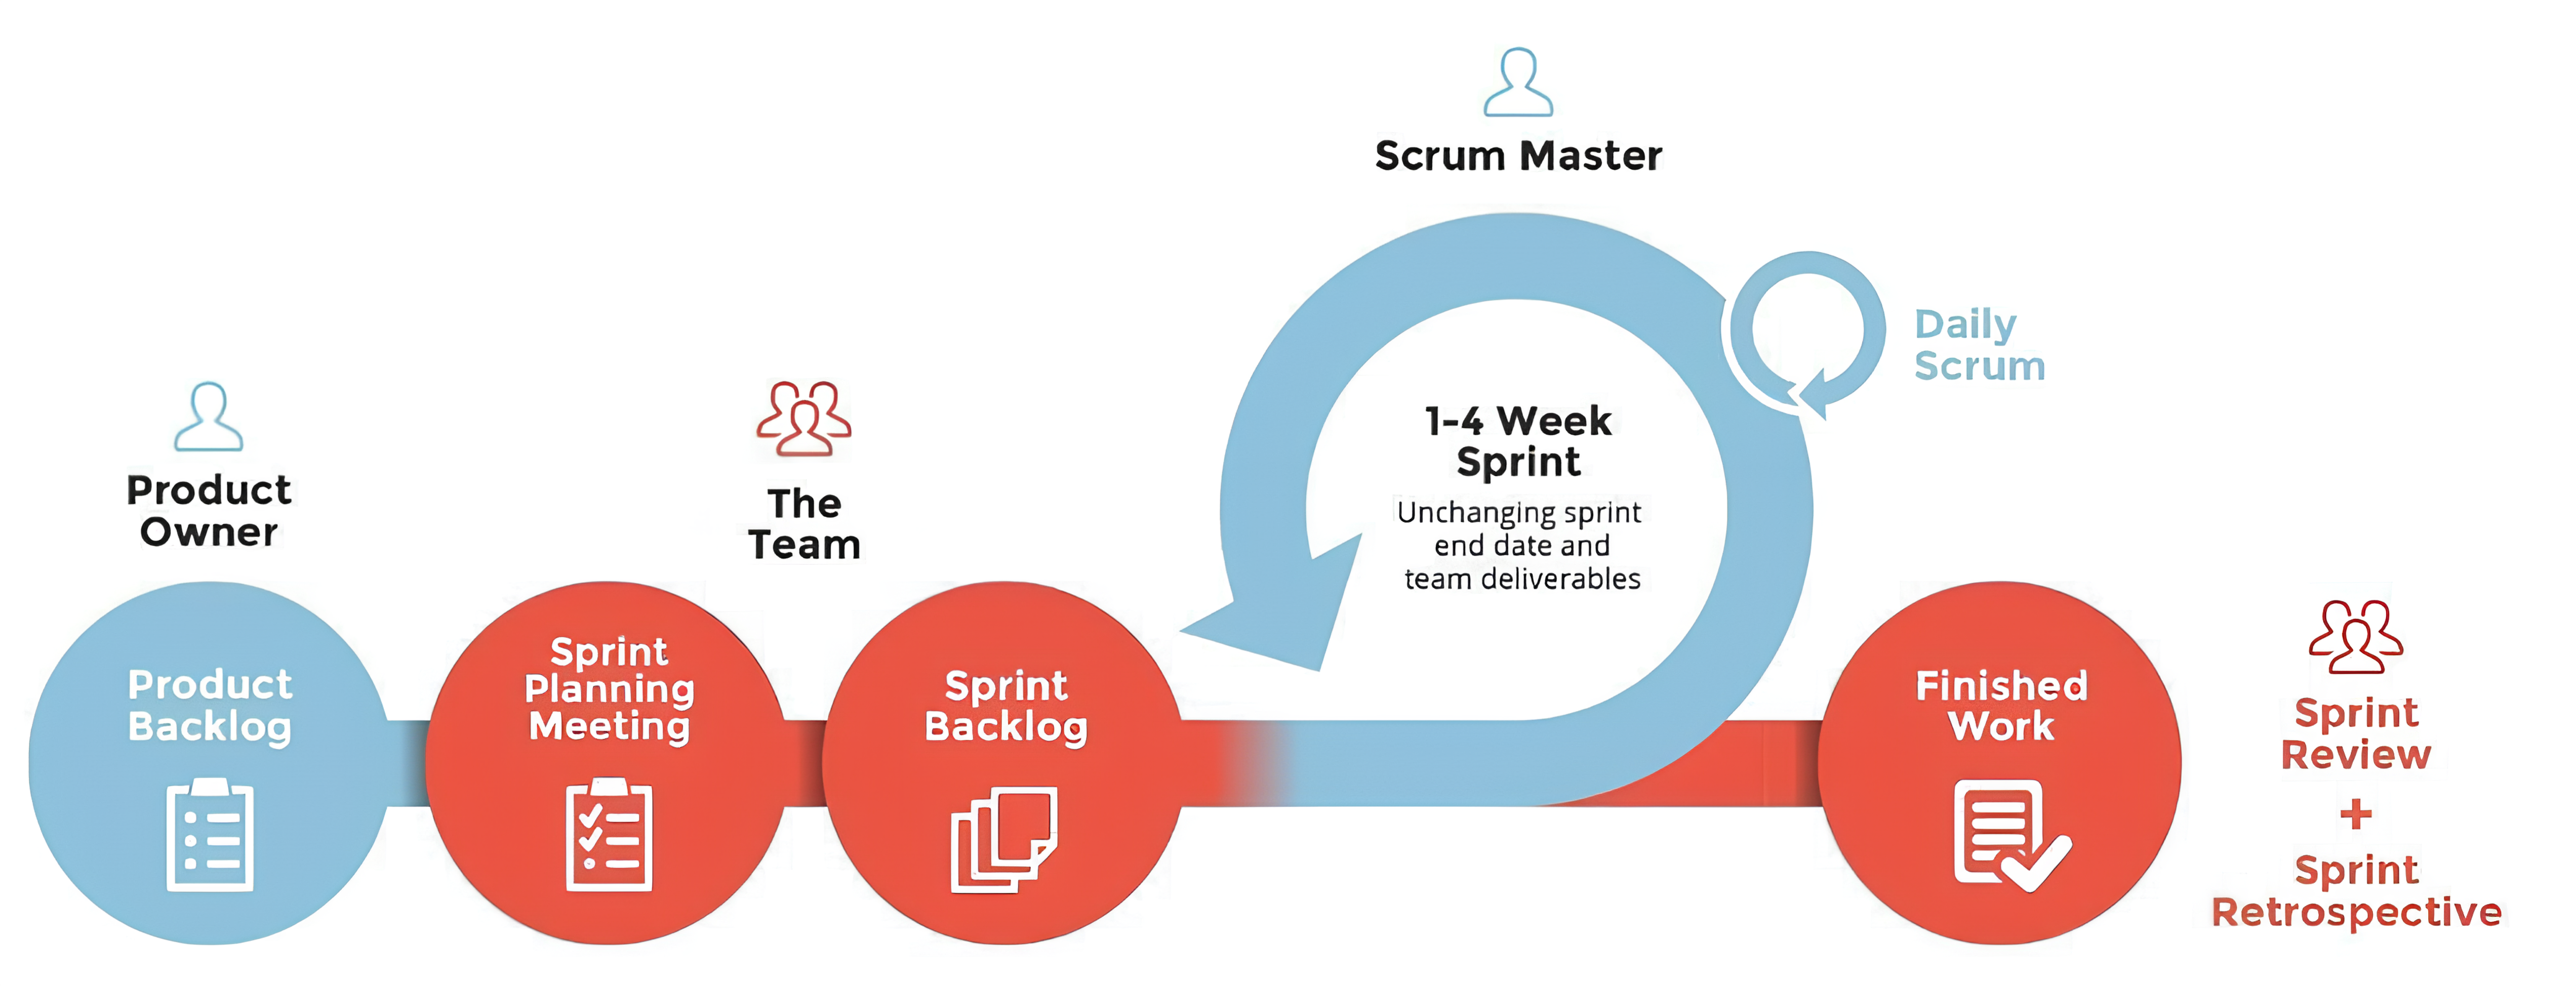
\includegraphics[width=1\textwidth]{images/scrum.png}
    \caption{Processus de SCRUM}
    \label{fig:scrum}
\end{figure}

% \subsection{Equipes et rôles}

% La répartition des rôles au sein de l’équipe projet, selon l’approche Scrum, est présentée dans le tableau \ref{tab:equipe_roles}.\\

% \begin{minipage}{1\textwidth}
%     \centering
% \begin{tabular}{|c|>{\raggedright\arraybackslash}p{10cm}|}
%   \hline
%   Product Owner &  \\
%   \hline
%   Scrum Master &  \\
%   \hline
%   L'équipe de développement & 
%    \\
%   \hline
% \end{tabular}
% \captionof{table}{Équipes et rôles}
% \label{tab:equipe_roles}
% \end{minipage}

\subsection{Planification du projet}
La phase de planification revêt une importance capitale dans la préparation d’un projet. Elle implique l’identification et la planification des différentes tâches du projet, ainsi que l’estimation de leur charge de travail respective. 

Le découpage temporel du projet en sprints, ainsi que les activités principales associées à chaque phase, sont présentés dans le tableau \ref{tab:planification}.

\begin{table}[h!]
\centering
\begin{tabularx}{\textwidth}{|c|X|}
  \hline
  \textbf{Période} & \textbf{Sprint / Activités} \\
  \hline
  2 semaines & Sprint 1 : Prise en main du sujet et compréhension du besoin  \\
  \hline
  1 semaine & Sprint 2 : Ingestion et couche Bronze \\
  \hline
  1 semaine & Sprint 3 : Transformation et couches Argent/Or  \\
  \hline
  2 semaines & Sprint 4 : Pipeline de classification et inférence  \\
  \hline
  1 semaines & Sprint 5 : Visualisation des données  \\
  \hline
  1 semaines & Sprint 6 : Phase de test et validation des résultats \\
  \hline
\end{tabularx}
\caption{Planification du projet}
\label{tab:planification}
\end{table}

\subsection{Synthèse visuelle}
\subsubsection{Diagramme de GANTT}
La planification globale du projet, incluant la répartition des tâches dans le temps, est visualisée à travers le diagramme de Gantt présenté à la figure \ref{fig:gantt}. Ce dernier constitue l’un des outils les plus efficaces pour représenter l’état d’avancement des différentes tâches qui composent un projet. Les unités de temps (jours, semaines, mois) sont indiquées en haut du diagramme, tandis que toutes les tâches à accomplir apparaissent dans la colonne de gauche. Chaque tâche est représentée par une barre horizontale dont la position et la longueur indiquent respectivement la date de début, la durée et la date de fin. Ce diagramme permet ainsi de visualiser clairement l’enchaînement des activités, leur durée, ainsi que les dates clés du projet.

\begin{figure}[H]
    \centering
    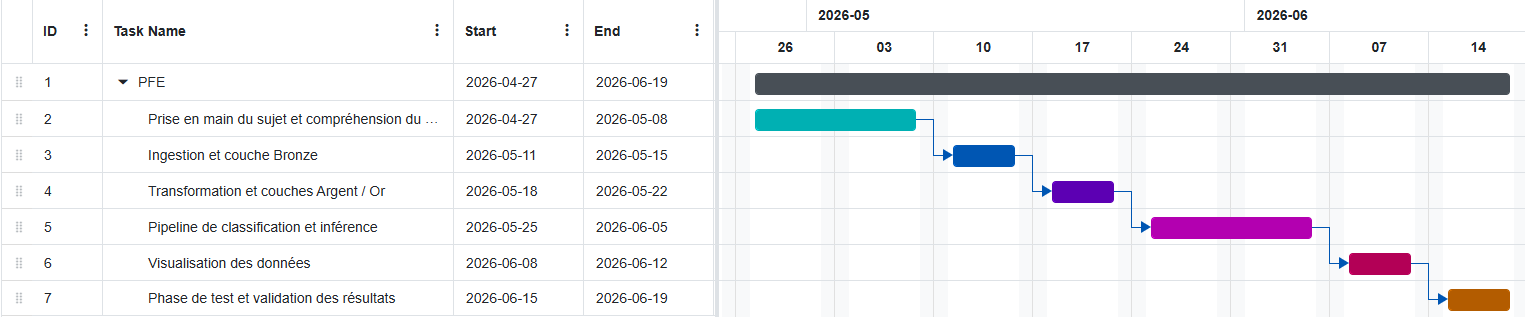
\includegraphics[width=1\textwidth]{images/gantt.png}
    \caption{Diagrmme de Gantt}
    \label{fig:gantt}
\end{figure}

%------------------------9-------------------------

\section{Conclusion}
Ce chapitre a permis de délimiter le périmètre du projet en posant le contexte métier, en analysant les approches existantes et en formulant la problématique à laquelle nous répondons. La solution retenue, ses objectifs, ses livrables et ses exigences ont été exposés de manière détaillée, et la démarche de conduite du projet a été établie. Dans le chapitre suivant, nous dresserons un état de l'art des concepts et technologies liés au Big Data, en justifiant les choix techniques retenus pour la réalisation de la plateforme
